\documentclass[11pt,a4paper,reqno,final]{article}
\usepackage{amsmath,amsfonts,amssymb}
\usepackage[table,xcdraw]{xcolor}
\usepackage{tikz}
\usepackage[colorlinks=true,breaklinks=true,linkcolor=lightblue,citecolor=lightgreen,urlcolor=lightblue]{hyperref}

\begin{document}

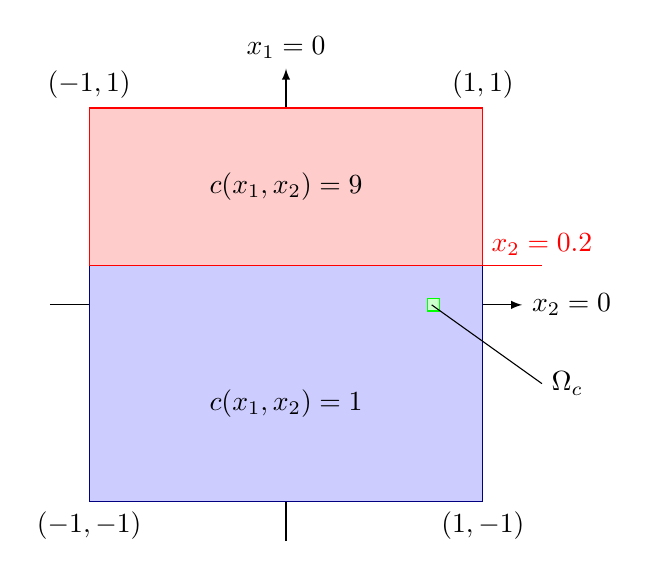
\begin{tikzpicture}[scale=2.5, >=latex]
    % Set the aspect ratio to ensure the domain appears square
    \draw[->] (-1.2,0) -- (1.2,0) node[right] {$x_2=0$};
    \draw[->] (0,-1.2) -- (0,1.2) node[above] {$x_1=0$};

    % Draw the shaded regions
    \filldraw[fill=blue!20, draw=blue!50!black] (-1,-1) rectangle (1,0.2);
    \filldraw[fill=red!20, draw=red!50!red] (-1,0.2) rectangle (1,1);
    \filldraw[fill=green!20, draw=green!50!green] (0.71875,-0.03125) rectangle (0.78125,0.03125);

    % Draw the line x2 = 0.2
    \draw[red] (-1,0.2) -- (1.3,0.2) node[above] {$x_2=0.2$};
    \draw[black] (0.74,0) -- (1.3,-0.4) node[right] {$\Omega_c$};
    % Label the regions
    \node at (0,0.6) {$c(x_1,x_2) = 9$};
    \node at (0,-0.5) {$c(x_1,x_2) = 1$};
    
    % Labels for the lines
    \node[below] at (-1,-1) {$(-1,-1)$};
    \node[below] at (1,-1) {$(1,-1)$};
    \node[above] at (-1,1) {$(-1,1)$};
    \node[above] at (1,1) {$(1,1)$};
\end{tikzpicture}

\end{document}